\section{Neural Networks as Function Approximators}
Will come soon \ldots

The aim is to approximate a solution to the differential equation described in the previous chapter.  

Perceptron

\begin{figure}[H]
    \begin{center}
        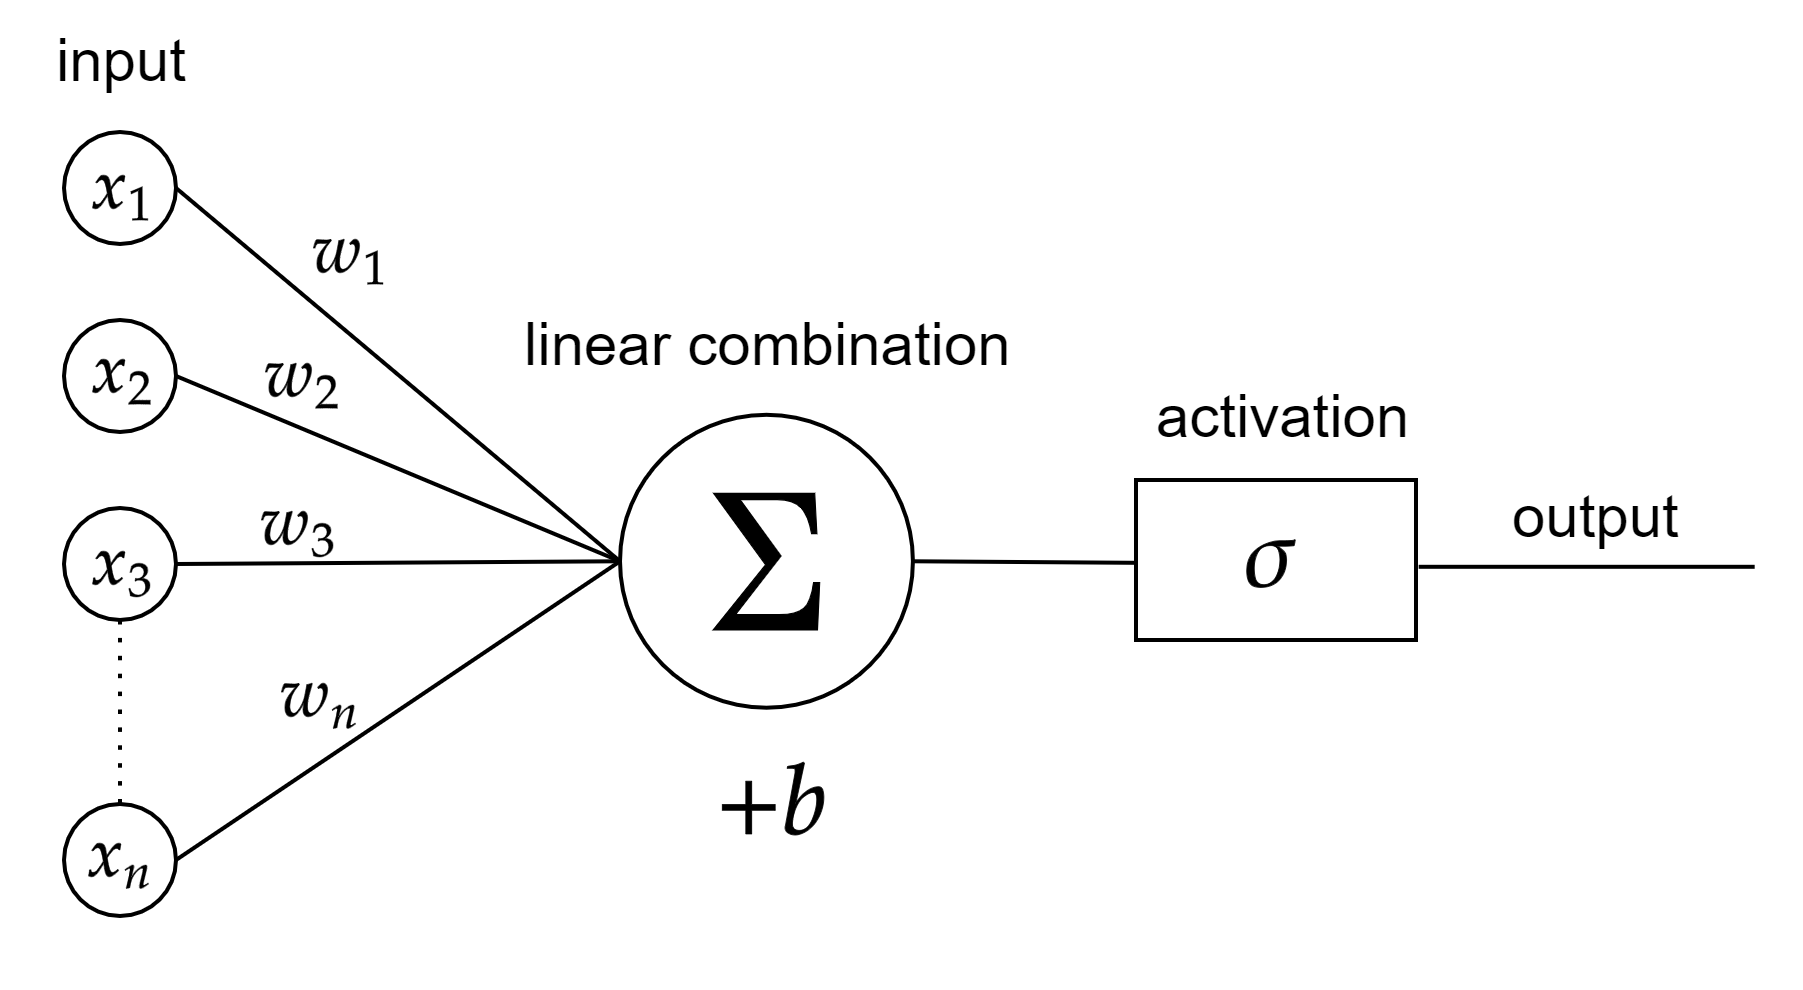
\includegraphics[scale=0.3]{img/diagram-20220205_1.png}
    \end{center}
    \caption{Illustration of the perceptron model for a single neuron.}
    \label{fig4}
\end{figure}



Deep-learning methods are 
representation-learning methods with multiple levels of representation, obtained by composing simple but non-linear modules that each 
transform the representation at one level (starting with the raw input) 
into a representation at a higher, slightly more abstract level. With the 
composition of enough such transformations, very complex functions 
can be learned.

The most common form of machine learning, deep or not, is supervised learning.

The 
equations used for computing the forward pass in a neural net

The non-linear functions used in neural networks include the rectified 
linear unit, commonly used in recent years, as 
well as the more conventional sigmoids, such as the hyberbolic tangent, 

We compute an objective function that measures the error (or distance) between the output scores and the desired pattern of scores. The 
machine then modifies its internal adjustable parameters to reduce 
this error. These adjustable parameters, often called weights, are real 
numbers that can be seen as ‘knobs’ that define the input–output function of the machine. In a typical deep-learning system, there may be 
hundreds of millions of these adjustable weights, and hundreds of 
millions of labelled examples with which to train the machine. 
To properly adjust the weight vector, the learning algorithm computes a gradient vector that, for each weight, indicates by what amount 
the error would increase or decrease if the weight were increased by a 
tiny amount. The weight vector is then adjusted in the opposite direction to the gradient vector. 

A deep-learning architecture is a multilayer stack of simple modules, all (or most) of which are subject to learning, and many of which 
compute non-linear input–output mappings. Each module in the 
stack transforms its input to increase both the selectivity and the 
invariance of the representation.

The backpropagation procedure to compute the gradient of an 
objective function with respect to the weights of a multilayer stack 
of modules is nothing more than a practical application of the chain rule for derivatives. The key insight is that the derivative (or gradient) of the objective with respect to the input of a module can be 
computed by working backwards from the gradient with respect to 
the output of that module

Many applications of deep learning use feedforward neural network architectures (Fig. 1), which learn to map a fixed-size input 
(for example, an image) to a fixed-size output (for example, a probability for each of several categories). To go from one layer to the 
next, a set of units compute a weighted sum of their inputs from the 
previous layer and pass the result through a non-linear function. At 
present, the most popular non-linear function is the rectified linear 
unit (ReLU), which is simply the half-wave rectifier. 
In past decades, neural nets used smoother non-linearities, such as 
, but the ReLU typically learns much faster 
in networks with many layers, allowing training of a deep supervised 
network without unsupervised pre-training28. Units that are not in 
the input or output layer are conventionally called hidden units. The 
hidden layers can be seen as distorting the input in a non-linear way 
so that categories become linearly separable by the last layer 

Perceptron
Activation Function
Neural Network
FNN
ResNet
Machine Learning, Training 
Supervised Learning
Unsupervised Learning
Gradient Based optimization
Backpropagation 
Honrik 